
\section{Assertions}
\begin{frame}{\textbf{Assertions}}
    Assertions are statements that check if some predicate holds. 
    Assertions help make sure that a program is always in a valid state.
    If an assertion fails, a program crash is triggered.
    \begin{block}{Assertion Types}
        There is usually a couple of categories of assertions.
        \begin{itemize}
            \item \textbf{Pre-Condition}: assertions that must hold before a function or procedure is called. 
                                        Ensures that call is made with valid args.
            \item \textbf{Post Conditions}: assertions that must hold after a procedure/function.
                                           e.g. return type, valid result, etc.
            \item \textbf{Invariants}: assertions that must always hold, e.g some var is always above a certain value.
        \end{itemize}
    \end{block}
\end{frame}

%\section*{Slutt}
\begin{frame}
    \begin{center}
        \begin{Large}
        \textbf{Lykke til på eksamen!\\[5mm]
        Takk for meg :)}
        
        \end{Large}
        \begin{figure}
            \centering
            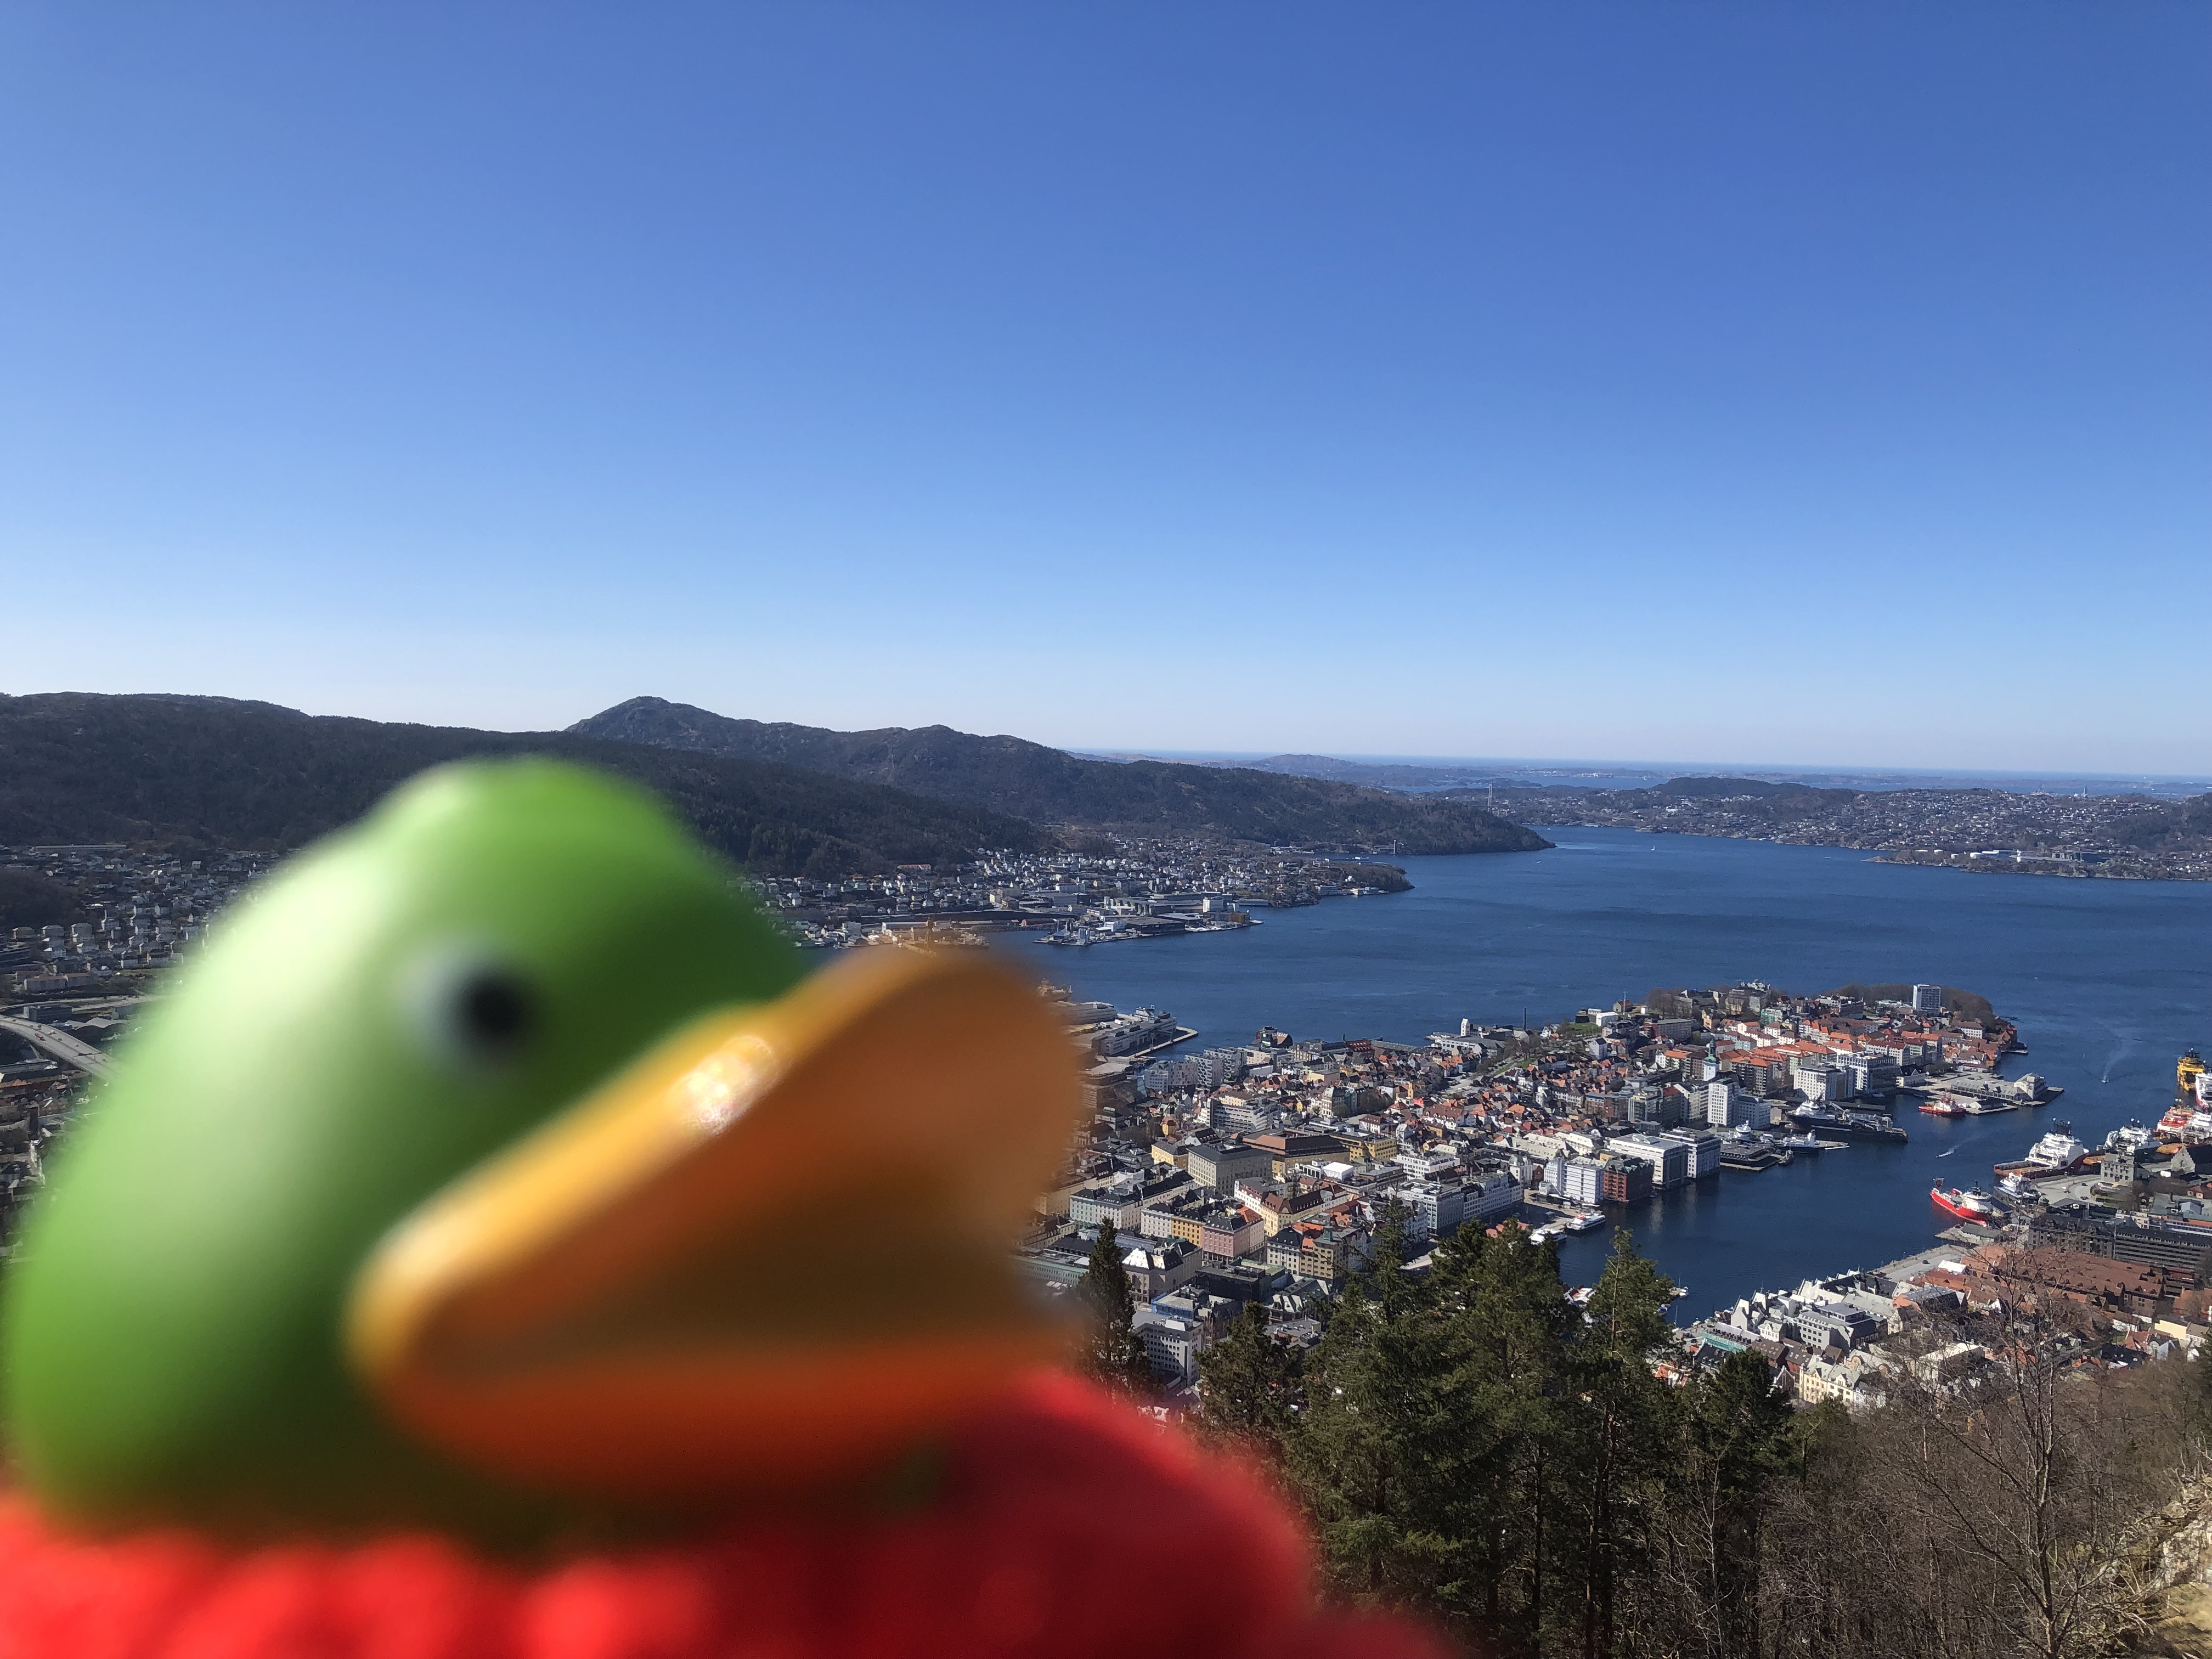
\includegraphics[height = 4.9cm]{guillaume10.jpg}
        \end{figure}
    \end{center}  
\end{frame}